\documentclass[hidelinks,12pt]{article}
\usepackage[left=0.25cm,top=1cm,right=0.25cm,bottom=1cm]{geometry}
%\usepackage[landscape]{geometry}
\textwidth = 20cm
\hoffset = -1cm
\usepackage[utf8]{inputenc}
\usepackage[spanish,es-tabla]{babel}
\usepackage[autostyle,spanish=mexican]{csquotes}
\usepackage[tbtags]{amsmath}
\usepackage{nccmath}
\usepackage{amsthm}
\usepackage{amssymb}
\usepackage{mathrsfs}
\usepackage{graphicx}
\usepackage{subfig}
\usepackage{standalone}
\usepackage[outdir=./Imagenes/]{epstopdf}
\usepackage{siunitx}
\usepackage{physics}
\usepackage{color}
\usepackage{float}
\usepackage{hyperref}
\usepackage{multicol}
%\usepackage{milista}
\usepackage{anyfontsize}
\usepackage{anysize}
%\usepackage{enumerate}
\usepackage[shortlabels]{enumitem}
\usepackage{capt-of}
\usepackage{bm}
\usepackage{relsize}
\usepackage{placeins}
\usepackage{empheq}
\usepackage{cancel}
\usepackage{wrapfig}
\usepackage[flushleft]{threeparttable}
\usepackage{makecell}
\usepackage{fancyhdr}
\usepackage{tikz}
\usepackage{bigints}
\usepackage{scalerel}
\usepackage{pgfplots}
\usepackage{pdflscape}
\pgfplotsset{compat=1.16}
\spanishdecimal{.}
\renewcommand{\baselinestretch}{1.5} 
\renewcommand\labelenumii{\theenumi.{\arabic{enumii}})}
\newcommand{\ptilde}[1]{\ensuremath{{#1}^{\prime}}}
\newcommand{\stilde}[1]{\ensuremath{{#1}^{\prime \prime}}}
\newcommand{\ttilde}[1]{\ensuremath{{#1}^{\prime \prime \prime}}}
\newcommand{\ntilde}[2]{\ensuremath{{#1}^{(#2)}}}

\newtheorem{defi}{{\it Definición}}[section]
\newtheorem{teo}{{\it Teorema}}[section]
\newtheorem{ejemplo}{{\it Ejemplo}}[section]
\newtheorem{propiedad}{{\it Propiedad}}[section]
\newtheorem{lema}{{\it Lema}}[section]
\newtheorem{cor}{Corolario}
\newtheorem{ejer}{Ejercicio}[section]

\newlist{milista}{enumerate}{2}
\setlist[milista,1]{label=\arabic*)}
\setlist[milista,2]{label=\arabic{milistai}.\arabic*)}
\newlength{\depthofsumsign}
\setlength{\depthofsumsign}{\depthof{$\sum$}}
\newcommand{\nsum}[1][1.4]{% only for \displaystyle
    \mathop{%
        \raisebox
            {-#1\depthofsumsign+1\depthofsumsign}
            {\scalebox
                {#1}
                {$\displaystyle\sum$}%
            }
    }
}
\def\scaleint#1{\vcenter{\hbox{\scaleto[3ex]{\displaystyle\int}{#1}}}}
\def\bs{\mkern-12mu}


%\usepackage{showframe}
\usepackage{apacite}
\title{Funciones de Chebychev \\ \large {Tema 5 - Funciones especiales} \vspace{-3ex}}
\author{M. en C. Gustavo Contreras Mayén}
\date{ }
\begin{document}
\vspace{-4cm}
\maketitle
\fontsize{14}{14}\selectfont
\tableofcontents
\newpage
%Referencia Riley 18.4 Chebyshev functions
\section{Funciones de Chebychev.}
La ecuación diferencial de Chebychev tiene la forma:
\begin{align}
(1 - x^{2}) \, \stilde{y} - x \, \ptilde{y} + \nu^{2} \, y
 = 0
 \label{eq:ecuacion_18_054}
\end{align}
y tiene tres puntos singulares regulares, en $x = -1, 1, \infty$. Al comparar la ecuación con
\begin{align*}
(1 - x^{2}) \, \stilde{y} - x \, \ptilde{y} + \ell (\ell + 1) \, y = 0
\end{align*}
vemos que la ecuación de Chebyshev es muy similar en forma a la ecuación de Legendre. A pesar de esta similitud, la ecuación (\ref{eq:ecuacion_18_054}) no se presenta con mucha frecuencia en problemas físicos, aunque \emph{sus soluciones son de considerable importancia en el análisis numérico}.
\par
El parámetro $\nu$ es un número real dado, pero en casi todas las aplicaciones prácticas toma un valor entero. De aquí en adelante asumimos que $\nu = n$, donde $n$ es un número entero no negativo. Como fue el caso de la ecuación de Legendre, en el uso normal la variable $x$ es el coseno de un ángulo, por lo que $-1 \leq x \leq 1$. Cualquier solución de la ec. (\ref{eq:ecuacion_18_054}) se llama \emph{función de Chebyshev}.
\par
El punto $x = 0$ es un punto ordinario de la ec. (\ref{eq:ecuacion_18_054}), por lo que esperamos encontrar
dos soluciones linealmente independientes de la forma
\begin{align*}
y = \sum_{m=0}^{\infty} a_{m} \, x^{m}
\end{align*}
Se podrían encontrar las relaciones de recurrencia para los coeficientes $a_{m}$ de una manera similar a la utilizada para la ecuación de Legendre. Para la ecuación de Chebyshev, sin embargo, es más fácil y esclarecedor adoptar un enfoque diferente. En particular, notamos que, al hacer la sustitución $x = \cos \theta$, y en consecuencia
\begin{align*}
\dv{x} = \left( \dfrac{-1}{\sin \theta} \right) \, \dv{\theta}
\end{align*}
la ecuación de Chebyshev se convierte en (con $\nu = n$):
\begin{align*}
\dv[2]{y}{\theta} + n^{2} \, y = 0
\end{align*}
que corresponde a la ecuación del oscilador armónico simple, con solución $\cos n \theta$ y $\sin n \theta$. 
\par
Las correspondientes soluciones linealmente independientes de la ecuación de Chebyshev están dadas por:
\begin{align}
\begin{aligned}
T_{n} (x) &= \cos (n \, \cos^{-1} x) \\[0.5em]
V_{n} (x) &= \sin (n \, \cos^{-1} x)
\end{aligned}
\label{eq:ecuacion_18_055}
\end{align}
Es sencillo demostrar que los $T_{n} (x)$ son polinomios de orden $n$, mientras que $V_{n} (x)$ no son polinomios.
\subsection{Forma explícita de \texorpdfstring{{$T_{n}(x)$}{}} y \texorpdfstring{{$V_{n}(x)$}{}} .}

Escribiendo $x = \cos \theta$, conviene primero formar la superposición compleja
\begin{align*}
T_{n}(x) + i \, V_{n} (x) &= \cos n \theta + i \, \sin n \theta = \\[0.5em]
&= (\cos \theta + i \, \sin \theta)^{n} = \\[0.5em]
&= \left( x + i \, \sqrt{1- x^{2}} \right)^{n} \hspace{1.5cm} \mbox{para  } \abs{x} \leq 1
\end{align*}
Entonces, al expandir la última expresión con el teorema binomial, obtenemos:
\begin{align}
T_{n}(x) = x^{n} - \binom{n}{2} \, x^{n-2} \, (1 - x^{2}) + \binom{n}{4} \, x^{n-4} \, (1 - x^{2})^{2} - \ldots \label{eq:ecuacion_18_056}
\end{align}
\begin{align}
\begin{aligned}[b]
V_{n}(x) &= \sqrt{1 - x^{2}} \, \bigg[ \binom{n}{1} \, x^{n-1} - \binom{n}{3} \, x^{n-3} \, (1- x^{2}) + \\[0.5em]
&+ \binom{n}{5} \, x^{n-5} \, (1- x^{2})^{2} + \ldots \bigg]
\end{aligned}
\label{eq:ecuacion_18_057}
\end{align}
De esta manera vemos que $T_{n}(x)$ es un polinomio de orden $n$, pero $V_{n}(x)$ no es un polinomio.

\subsection{Funciones adicionales.}

Es conveniente definir las funciones adicionales:
\begin{align}
\begin{aligned}
W_{n} (x) &= (1 - x^{2})^{-1/2} \, T_{n+1} (x) \\[0.5em]
U_{n} (x) &= (1 - x^{2})^{-1/2} \, V_{n+1} (x)
\end{aligned}
\label{eq:ecuacion_18_058}
\end{align}
De las ecs. (\ref{eq:ecuacion_18_056}) y (\ref{eq:ecuacion_18_057}), vemos de inmediato que $U_{n}(x)$ es un \emph{polinomio de orden n}, mientras que $W_{n}(x)$ no lo es.
\par
En la práctica, es habitual trabajar íntegramente en términos de los $T_{n} (x)$ y $U_{n} (x)$, que se conocen, respectivamente, como los \emph{polinomios de Chebyshev de primer y segundo tipo}. En particular, observamos que la solución general de la ecuación de Chebyshev se puede escribir en términos de estos polinomios como:
\begin{align*}
y(x) = \begin{cases}
c_{1} \, T_{n} (x) + c_{2} \, \sqrt{1 -x^{2}} \, U_{n-1} (x) & \mbox{para  } n = 1, 2, 3, \ldots \\[0.5em]
c_{1} + c_{2} \, \sin^{-1} x & \mbox{para  } n = 0
\end{cases}
\end{align*}
La solución con $n = 0$ se puede escribir como:
\begin{align*}
d_{1} + c_{2} \, \cos^{-1} x \hspace{1.5cm} \mbox{con  } d_{1} = c_{1} + \dfrac{1}{2} \, \pi \, c_{2}
\end{align*}
Los primeros polinomios de Chebychev de primer tipo se pueden construir fácilmente y están dado por:
\begin{table}[H]
\centering
\fontsize{14}{14}\selectfont
\begin{tabular}{p{6cm} p{6cm}}
$T_{0}(x) = 1$ & $T_{1} = x$ \\[0.5em]
$T_{2}(x) = 2 \, x^{2} - 1$ & $T_{3} = 4 \, x^{3} - 3 \, x$ \\[0.5em]
$T_{4}(x) = 8 \, x^{4} - 8 \, x^{2} + 1$ & $T_{5} = 16 \, x^{5} - 20 \, x^{3} + 5 \, x$ \\[0.5em]
\vdots & \vdots
\end{tabular}
\end{table}
En la figura (\ref{fig:figura_plot_chebychev_01}) se presenta la gráfica de los primeros polinomios de Chebychev de primera clase.
\begin{figure}[H]
    \centering
    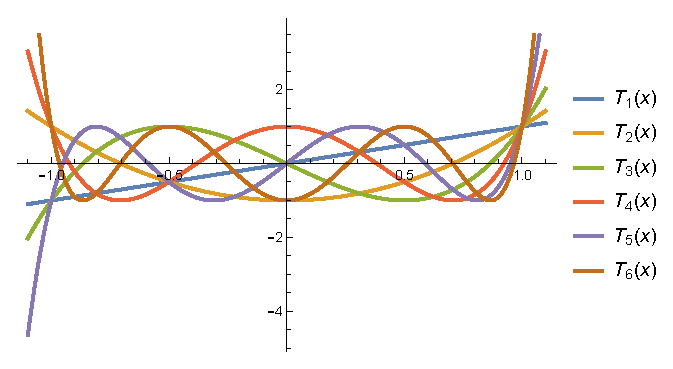
\includegraphics[scale=1]{Imagenes/Plot_Polinomios_Chebychev_01.eps}
    \caption{Primeros polinomios de Chebychev de primera clase.}
    \label{fig:figura_plot_chebychev_01}
\end{figure}
En general, los polinomios de Chebychev $T_{n}(x)$ satisfacen:
\begin{align*}
T_{n}(-x) = (-1)^{n} \, T_{n} (x)
\end{align*}
que se puede deducir fácilmente a partir de la ec. (\ref{eq:ecuacion_18_056}). También es fácil deducir los siguientes valores especiales:
\begin{align*}
T_{n} (1) &= 1 \\[0.5em]
T_{n} (-1) &= (-1)^{n} \\[0.5em]
T_{2n} (0) &= (-1)^{n} \\[0.5em]
T_{2n+1} (0) &= 0
\end{align*}
Los primeros polinomios de Chebychev de segunda clase se pueden obtener fácilmente, se presentan a continuación los primeros:
\begin{table}[H]
\centering
\fontsize{14}{14}\selectfont
\begin{tabular}{p{6cm} p{6cm}}
$U_{0}(x) = 1$ & $U_{1} = 2 \, x$ \\[0.5em]
$U_{2}(x) = 4 \, x^{2} - 1$ & $U_{3} = 8 \, x^{3} - 4 \, x$ \\[0.5em]
$U_{4}(x) = 16 \, x^{4} - 12 \, x^{2} + 1$ & $U_{5} = 32 \, x^{5} - 32 \, x^{3} + 6 \, x$ \\[0.5em]
\vdots & \vdots
\end{tabular}
\end{table}
Las funciones que representan a los polinomios de Chebychev de segunda clase se presentan en la figura (\ref{fig:figura_plot_chebychev_02}):
\begin{figure}[H]
    \centering
    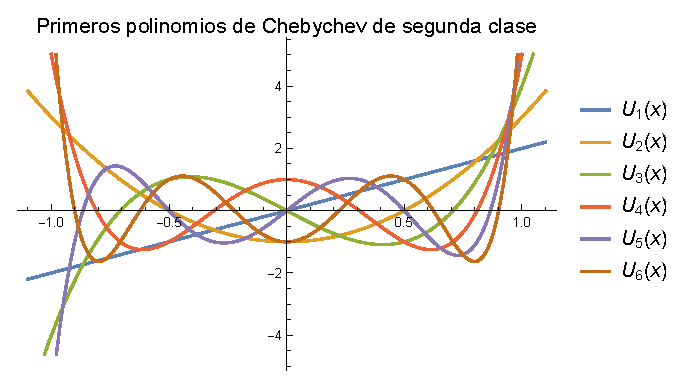
\includegraphics[scale=1]{Imagenes/Plot_Polinomios_Chebychev_02.eps}
    \caption{Primeros polinomios de Chebychev de segunda clase.}
    \label{fig:figura_plot_chebychev_02}
\end{figure}
Los polinomios de Chebychev $U_{n}(x)$ también satisfacen la propiedad:
\begin{align*}
U_{n} (-x) = (-1)^{n} \, U_{n} (x)
\end{align*}
la cual se puede deducir de las ecs. (\ref{eq:ecuacion_18_057}) y (\ref{eq:ecuacion_18_058}), y tiene, entre otros, los siguientes valores especiales:
\begin{align*}
U_{n} (1) &= n + 1 \\[0.5em]
U_{n} (-1) &= (-1)^{n} \, (n + 1) \\[0.5em]
U_{2n} (0) &= (-1)^{n} \\[0.5em]
U_{2n+1} (0) &= 0
\end{align*}

\section{Propiedades de los polinomios de Chebychev.}

\end{document}